
% %NOTE:
% % CHECKED WITH SLIDES: YES!
% % CHECKED WITH EXERCISES: NO -- TODO
% % MISSING: Stuff about internet of things and trends -- but left out since not relevant

\section{Architecture Design}

\subsection{Task Graph/Dependence Graph/Data Flow Graph}
\begin{theorem}[Task Graph or Dependence Graph (DG)]

A dependence graph is a directed graph $G=(V,E)$ in which $E \subseteq V \times V$ is a partial order.

If $(v1, v2) \in E$, then v1 is called an immediate predecessor of v2 and v2 is called an immediate successor of v1.

Suppose $E^*$ is the transitive closure of E. If $(v1, v2) \in E^*$, then v1 is called a predecessor of v2 and v2 is called a successor of v1.

\end{theorem}

\begin{itemize}[noitemsep]
\item A dependence graph describes order relations for the execution of single operations or tasks. Nodes correspond to tasks or operations, edges correspond to relations („executed after“). 
\item Usually, a dependence graph describes a partial order between operations and therefore, leaves freedom for scheduling (parallel or sequential). It represents parallelism in  a program but no branches in control flow
\item A dependence graph is acyclic
\item A dependence graph cannot handle branches
\end{itemize}


\subsection{Control-Data Flow Graph (CDFG)}

\begin{itemize}[noitemsep]
\item Goal: Description of control structures (for example branches) and 
data dependencies
\item Applications: Describing the semantics of programming languages, internal representation in compilers for hardware and software
\item Representation: Combination of control flow (sequential state machine) using the CFG and dependence representation using DFG
\end{itemize}

\subsubsection{Control Flow Graph (statement transitions)}
\begin{itemize}[noitemsep]
\item corresponds to a finite state machine, which represents the sequential control flow in a program
\item Branch conditions are very often associated to the outgoing edges of a node. 
\item The operations to be executed within a state (node) are associated in form of a dependence graph
\end{itemize}

\subsubsection{Data Flow Graph (statement dependence)}
NOP (no operation) operations represent the start point and 
end point of the execution. This form of a graph is called a 
polar graph: it contains two distinguished nodes, one without incoming edges, the other one without outgoing edges

\begin{figure}[ht]
	\centering
  	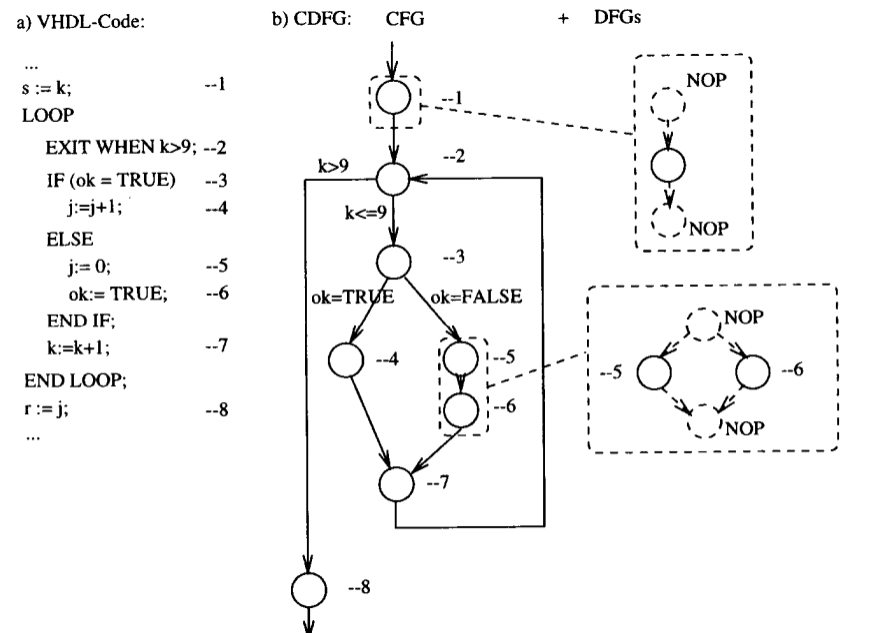
\includegraphics[scale=0.4]{img/10_CDFG.png}
	\caption{An example of a CDFG graph}
	\label{fig_CDFG_graph}
\end{figure}

\subsection{Sequence Graph (SG)}

A sequence graph is a hierarchy of directed graphs. A 
generic element of the graph is a dependence graph with the following properties

\begin{itemize}[noitemsep]
\item It contains two kinds of nodes: (a) operations or tasks
and (b) hierarchy nodes
\item Each graph is acyclic and polar with two distinguished nodes: the start node and the end node. No operation is assigned to them (NOP)
\item There are the following hierarchy nodes: (a) module call (CALL) (b) branch (BR) and (c) iteration (LOOP)
\end{itemize}

\begin{tnote}
A hierarchical sequence graph can be cyclic.
\end{tnote}

\subsubsection{Example}

\begin{lstlisting}[basicstyle=\small]
x := a * b;
y := x * c;
z := a + b;
IF z > 0 THEN
	p := m + n;
	q := m * n;
END IF
\end{lstlisting}


\begin{figure}[ht]
	\centering
  	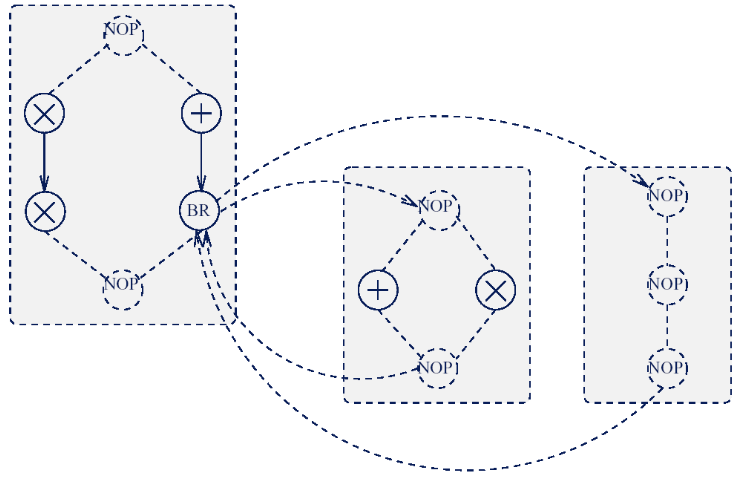
\includegraphics[scale=0.4]{img/10_example_sequence_graph.png}
	\caption{An example of a sequence graph. The edges to the if-else part are labelled with the condition or else}
	\label{fig_sequence_graph}
\end{figure}



\subsection{Resource Graph}
\begin{definition}[Resource Graph]
Resource Graph $G_R = (V_R, E_R), V_R = V_S \bigcup V_T$ where $V_S$ denotes the operations of the algorithm and $V_T$ the resource types of the architecture and $G_R$ is a biparpite graph. An edge $(v_s, v_t) \in E_R$ represents the availability of a resource type $v_t$ for an operation $v_s$.
\end{definition}

\begin{definition}[Cost function]
$c: V_T \rightarrow Z$
\end{definition}

\begin{definition}[Execution times]
$w: E_R \rightarrow Z \geq 0$ are assigned to each edge $(v_s, v_t) \in E_R$ and denote the execution time of operation $v_s \in V_S$ on resource type $v_t \in V_T$
\end{definition}



\subsection{Marked Graphs (MG)}
\begin{definition}[Marked Graph]
A marked graph $G = (V, A, del)$ consists of nodes (actors) $v \in V$, edges $a = (v_i, v_j ) \in A, A \subseteq V \times V$, number of initial tokens on edges $del: A \rightarrow N$. 

The marking (distribution of tokens) is often represented in a form of a vector. For an example, see figure \ref{fig_implementation_hw}.
\end{definition}


\begin{itemize}[noitemsep]
\item The token on the edges correspond to data that are stored in FIFO queues
\item A node (actor) is called activated if on every input edge there is at least one token
\item A node (actor) can fire if it is activated
\item The firing of a node $v_i$ (actor operates on the first tokens in the input queues) removes from each input edge a token and adds a token to each output edge. The output token correspond to the processed data
\item Marked graphs are mainly used for modeling 
regular computations, for example signal flow graphs.
\end{itemize}

\subsubsection{Implementation as a synchronous digital circuit}
\begin{itemize}[noitemsep]
\item Actors are implemented as combinatorial circuits
\item Edges correspond to synchronously clocked shift registers
\end{itemize}

\begin{figure}[ht]
	\centering
  	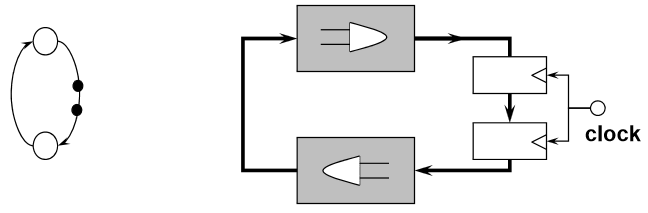
\includegraphics[scale=0.5]{img/10_implementation_hardware.png}
	\caption{Implemenation of a marked graph as a synchronous digital circuit}
	\label{fig_implementation_hw}
\end{figure}

\subsubsection{Implementation as a self-timed asynchronous 
circuit}
\begin{itemize}[noitemsep]
\item Actors and FIFO registers are implemented as independent units
\item The coordination and synchronization of firings is implemented using a handshake protocol
\item Delay insensitive direct implementation of the semantics of marked graphs
\end{itemize}

\subsubsection{Implementation in software (static scheduling)}
Software implementation with static scheduling

\begin{itemize}[noitemsep]
\item At first, a feasible sequence of actor firings is determined which ends in the starting state (initial distribution of tokens). 
\item This sequence is implemented directly in software
\end{itemize}

\subsubsection{Implementation in software (dynamic scheduling)}

\begin{itemize}[noitemsep]
\item Scheduling is done using a (real-time) operating system.
\item Actors correspond to threads (or tasks)
\item After firing (finishing the execution of the corresponding thread) the thread is removed from the set of ready threads and put into wait state
\item It is put into the ready state if all necessary input data are present
\item This mode of execution directly corresponds to the semantics of marked graphs. It can be compared with the self-timed hardware implementation. 
\end{itemize}

\cleardoublepage

